\documentclass[../main.tex]{subfiles}
\graphicspath{{\subfix{../images/}}, {\subfix{../}}}

\begin{document}
	\chapter{Dressed Graphene Hamiltonian in Reciprocal Space}
	
	\todo{Clean up this section}
	
	In the following chapter, the model Hamiltonian
	\begin{align}
		H_0 = &-t_{\mathrm{X}} \sum_{\langle ij \rangle, \sigma} d_{i, \sigma}^{\dagger} d_{j, \sigma}
		-t_{\mathrm{Gr}} \sum_{\langle ij \rangle, \sigma}
		c_{i, \sigma}^{(A), \dagger} c_{j, \sigma}^{(B)}
		+ V \sum_{i, \sigma} d_{i, \sigma}^{\dagger} c_{i, \sigma}^{(A)} + \mathrm{h.c.} \label{eq:EG-X model Hamiltonian non-interacting appendix}
	\end{align}
	will be treated to obtain the band structure. The first step is to write out the sums over nearest neighbors \(\langle i, j \rangle\) explicitly, writing \(\vb{\delta}_{\mathrm{X}}, \vb{\delta}_{\epsilon}\) (\(\epsilon = A, B\)) for the vectors to the nearest neighbors of the \(\mathrm{X}\) atoms and Graphene \(A, B\) sites.
	Doing the calculation for example of the \(\mathrm{X}\) atoms:
	\begin{align}
		-t_{\mathrm{X}} \sum_{\langle ij \rangle, \sigma} (d_{i, \sigma}^{\dagger} d_{j, \sigma} + d_{j, \sigma}^{\dagger} d_{i, \sigma})
		&= -\frac{t_X}{2} \sum_{i,\sigma} \sum_{\vb{\delta}_{\mathrm{X}}} d_{i, \sigma}^{\dagger} d_{i + \vb{\delta}_{\mathrm{X}}, \sigma}
		-\frac{t_X}{2} \sum_{j,\sigma} \sum_{\vb{\delta}_{\mathrm{X}}} d_{j, \sigma}^{\dagger} d_{j + \vb{\delta}_{\mathrm{X}}, \sigma} \label{eq:EG-X model X atoms nearest neighbor sum double counting} \\
		&= -t_X \sum_{i,\sigma} \sum_{\vb{\delta}_{\mathrm{X}}} d_{i, \sigma}^{\dagger} d_{i + \vb{\delta}_{\mathrm{X}}, \sigma} \label{eq:EG-X model X atoms nearest neighbours written out}
	\end{align}
	The factor \(\nicefrac{1}{2}\) in \cref{eq:EG-X model X atoms nearest neighbor sum double counting} is to account for double counting when going to the sum over all lattice sites \(i\).
	By relabeling \(j \to i\) in the second sum, the two sum are the same and \cref{eq:EG-X model X atoms nearest neighbours written out} is obtained.
	Using now the discrete Fourier transform
	\begin{align}
		c_{i} &= \frac{1}{\sqrt{N}} \sum_{\vb{k}} e^{\iu \vb{k} \vb{r}_{i}} c_{\vb{k}} ,\;
		c_{i}^{\dagger} = \frac{1}{\sqrt{N}} \sum_{\vb{k}} e^{-\iu \vb{k} \vb{r}_{i}} c_{\vb{k}}^{\dagger}
	\end{align}
	with the completeness relation
	\begin{equation}
		\sum_{i} e^{\iu \vb{k} \vb{r}_{i}} e^{-\iu \vb{k}^{\prime} \vb{r}_{i}} = N \delta_{\vb{k}, \vb{k}^{\prime}}
		\;,
	\end{equation}
	\cref{eq:EG-X model X atoms nearest neighbours written out} reads:
	\begin{align}
		-t_X \frac{1}{N} \sum_{i,\sigma} \sum_{\vb{\delta}_{\mathrm{X}}} d_{i, \sigma}^{\dagger} d_{i + \vb{\delta}_{\mathrm{X}}, \sigma}
		&= -t_X \frac{1}{N} \sum_{i,\sigma} \sum_{\vb{k}, \vb{k}^{\prime}, \vb{\delta}_{\mathrm{X}}} \left(e^{-\iu \vb{k} \vb{r}_i} d_{\vb{k}, \sigma}^{\dagger} \right) \left(e^{\iu \vb{k}^{\prime} \vb{r}_i} e^{\iu \vb{k}^{\prime} \vb{\delta}_{\mathrm{X}}} d_{\vb{k}^{\prime}, \sigma} \right) \\
		&= -t_X \frac{1}{N} \sum_{\vb{k}, \vb{k^{\prime}}, \vb{\delta}_{\mathrm{X}}, \sigma} d_{\vb{k}, \sigma}^{\dagger}   d_{\vb{k}^{\prime}, \sigma} e^{\iu \vb{k}^{\prime} \vb{\delta}_{\mathrm{X}}} \sum_{i} e^{-\iu \vb{k} \vb{r}_i} e^{\iu \vb{k}^{\prime} \vb{r}_i} \\
		&= -t_X \frac{1}{N} \sum_{\vb{k}, \vb{k^{\prime}}, \sigma}  d_{\vb{k}, \sigma}^{\dagger}  d_{\vb{k}^{\prime}, \sigma} \sum_{\vb{\delta}_{\mathrm{X}}} e^{\iu \vb{k}^{\prime} \vb{\delta}_{\mathrm{X}}} \left(N \delta_{\vb{k}, \vb{k}^{\prime}} \right)\\
		&= -t_X \sum_{\vb{k}, \sigma}  d_{\vb{k}, \sigma}^{\dagger}d_{\vb{k}, \sigma} \sum_{\vb{\delta}_{\mathrm{X}}} e^{\iu \vb{k} \vb{\delta}_{\mathrm{X}}} \;.
	\end{align}
	This part is now diagonal in \(\vb{k}\) space.
	The nearest neighbours vectors \(\vb{\delta}_{\mathrm{X}}\) for the \(\mathrm{X}\) atoms are the vectors \(\vb{\delta}_{AA, i}\) from \cref{sec:lattice-structure-of-graphene}.
	With that, the sum over \(\vb{\delta}_{\mathrm{X}}\) can be explicitly calculated:
	\todo{Correct exp expressions}
	\todo{Example for a vector product}
	\begin{align}
		f_{\mathrm{X}} (\vb{k}) &= -t_X \sum_{\vb{\delta}_{\mathrm{X}}} e^{\iu \vb{k} \vb{\delta}_{\mathrm{X}}} \\
		&= -t_X \left[ \exp\left(\iu a \left(\frac{k_x}{2} + \frac{\sqrt{3} k_y}{2}\right)\right)
		+ e^{\iu a k_x}
		+ e^{\iu a (\frac{k_x}{2} - \frac{\sqrt{3} k_y}{2})}
		\right. \\
		&+ \left. e^{\iu a (-\frac{k_x}{2} - \frac{\sqrt{3} k_y}{2})}
		+ e^{-\iu a k_x}
		+ e^{\iu a (-\frac{k_x}{2} + \frac{\sqrt{3} k_y}{2})} \right] \\
		&= -t_X \left( 2 \cos{(a k_x)} + 2 e^{\iu a \frac{\sqrt{3} k_y}{2}} \cos{(\frac{a}{2} k_x)} + 2 e^{-\iu a \frac{\sqrt{3} k_y}{2}} \cos{(\frac{a}{2} k_x)} \right) \\
		&= -2t_X \left( \cos{(a k_x)} + 2 \cos{(\frac{a}{2} k_x)} \cos{(\sqrt{3} \frac{ a}{2} k_y)} \right) \;.
	\end{align}
	The same can be done for the hopping between Graphene sites, for example :
	\begin{align}
		-t_{\mathrm{Gr}} \sum_{\langle ij \rangle, \sigma \sigma^{\prime}} c_{i, \sigma}^{(A), \dagger} c_{j, \sigma^{\prime}}^{(B)}
		&= -t_{\mathrm{Gr}} \sum_{i, \sigma \sigma^{\prime}} \sum_{\vb{\delta}_{AB}} c_{i, \sigma}^{(A), \dagger} c_{i + \vb{\delta}_{AB} , \sigma^{\prime}}^{(B)} \\
		&= -t_{\mathrm{Gr}} \sum_{\vb{k}, \sigma, \sigma^{\prime}}  c_{\vb{k}, \sigma}^{(A) \dagger} c_{\vb{k}, \sigma^{\prime}}^{(B)} \sum_{\vb{\delta}_{AB}} e^{\iu \vb{k} \vb{\delta}_{AB}}
	\end{align}
	We note \todo{Show that!}
	\begin{align}
		\sum_{\vb{\delta}_{AB}} e^{\iu \vb{k} \vb{\delta}_{AB}} = \left( \sum_{\vb{\delta}_{BA}} e^{\iu \vb{k} \vb{\delta}_{BA}} \right)^* = \sum_{\vb{\delta}_{BA}} e^{-\iu \vb{k} \vb{\delta}_{BA}}
	\end{align}
	and calculate
	\begin{align}
		f_{Gr} &= -t_{Gr} \sum_{\vb{\delta}_{AB}} e^{\iu \vb{k} \vb{\delta}_{AB}} \\
		&= -t_{Gr} \left(
		e^{\iu \frac{a}{\sqrt{3}} k_y} +
		e^{\iu \frac{a}{2\sqrt{3}} (\sqrt{3} k_x - k_y)} +
		e^{\iu \frac{a}{2\sqrt{3}} (-\sqrt{3} k_x - k_y)} \right) \\
		&= -t_{Gr} \left(
		e^{\iu \frac{a}{\sqrt{3}} k_y} +
		e^{-\iu \frac{a}{2\sqrt{3}} k_y} \left(
		e^{\iu \frac{a}{2} k_x} + e^{-\iu \frac{a}{2} k_x}
		\right) \right) \\
		&= -t_{Gr} \left(
		e^{\iu \frac{a}{\sqrt{3}} k_y} +
		2 e^{-\iu \frac{a}{2\sqrt{3}} k_y}
		\cos{(\frac{a}{2} k_x)} \right)
	\end{align}
	All together, we get:
	\begin{align}
		H_0 &= \sum_{\vb{k}, \sigma, \sigma^{\prime}} \begin{pmatrix} c_{k, \sigma}^{A, \dagger} & c_{k, \sigma}^{B, \dagger} & d_{k, \sigma}^{\dagger} \end{pmatrix}
		\begin{pmatrix}
			0 & f_{Gr} & V \\
			f_{Gr}^* & 0 & 0 \\
			V & 0 & f_{X}
		\end{pmatrix} \begin{pmatrix} c_{k, \sigma}^{A} \\ c_{k, \sigma}^{B} \\ d_{k, \sigma} \end{pmatrix}
		\label{eq:EG-X Hamiltonian non-interacting matrix appendix}
	\end{align}
	The band structure for the non-interacting EG-X model is easily obtained by diagonalising the matrix in eq.~\ref{eq:EG-X Hamiltonian non-interacting matrix}.
	This was done in fig.~\ref{fig:EG-X model non-interacting bands}.
	
	Values used for calculation:
	\begin{itemize}
		\item \(a_0 = 1\)
		\item \(t_{\mathrm{Gr}} = 1\)
		\item \(t_{\mathrm{X}} = 0.01\)
	\end{itemize}
	\(V\) is the control parameter.
	A range from \(V=0.1\) to \(V=2\) can be mapped onto materials in experiment.
	
	\begin{figure}[t]
		\centering
		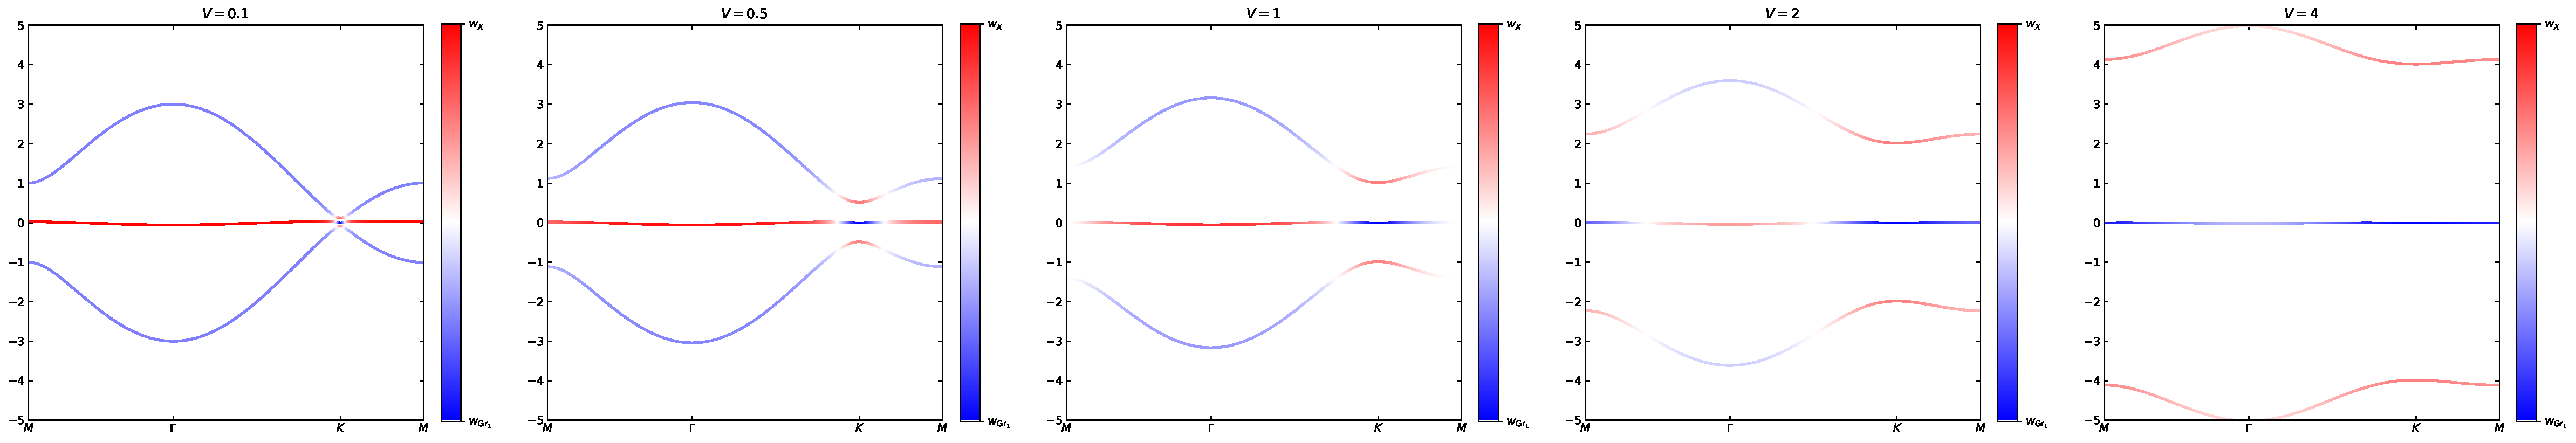
\includegraphics[width=\textwidth]{images/EG_X bands_tGr_1_tX_0.01}
		\caption{Bands of the non-interacting EG-X model. All the bands are spin-degenerate.}
		\label{fig:EG-X model non-interacting bands}
	\end{figure}
\end{document}